\chapter{Metodologia i~przygotowanie środowiska badawczego}

W~niniejszym rozdziale przedstawiono metodologię badawczą oraz szczegółowy opis przeprowadzonych eksperymentów. Ze względu na badawczy charakter pracy magisterskiej, główny nacisk położono na poprawne przeprowadzenie i~udokumentowanie procesu uczenia. Szczegółowo opisano również implementacje metod wykorzystywanych w~eksperymentach, co ma na celu ułatwienie potencjalnej replikacji uzyskanych wyników. W~pierwszej kolejności zdefiniowano założenia eksperymentalne, metryki ewaluacyjne oraz wykorzystaną infrastrukturę sprzętową opartą na akceleratorach graficznych wysokiej wydajności. Następnie opisano autorskie, zautomatyzowane środowisko programistyczne wykorzystane do zarządzania procesem uczenia. Rozdział zamyka szczegółowe omówienie algorytmów i~procedur zastosowanych do przygotowania danych treningowych, w~tym mechanizmów pseudoetykietowania oraz syntetycznego generowania obrazów tła.

\section{Założenia eksperymentalne i~metryki}

Celem przeprowadzonych eksperymentów była ocena wpływu technik uczenia półnadzorowanego (ang.\ \emph{Semi-Supervised Learning}, SSL), ze szczególnym uwzględnieniem iteracyjnego pseudoetykietowania oraz syntetycznej augmentacji danych, na zdolność generalizacji modeli detekcji obiektów.

Proces badawczy został podzielony na dwie główne fazy: ewaluację modeli odniesienia (ang.\ \emph{baseline}) wytrenowanych wyłącznie na małym zbiorze danych oraz uczenie modeli docelowych z~wykorzystaniem danych nieoznakowanych lub syntetycznych. W~badaniach wykorzystano trzy odrębne architektury:
\begin{itemize}
    \item \textbf{YOLOv8n} -- sprawdzony detektor jednoetapowy w~wariancie \emph{Nano},
    \item \textbf{YOLOv26n} -- nowszy, eksperymentalny wariant rodziny YOLO, optymalizujący efektywność parametrów w~wariancie \emph{Nano},
    \item \textbf{RT-DETR-L} -- oparty na transformerach wizyjnych detektor w~dużym wariancie (\emph{Large}). Wybór wariantu Large (około 32 mln parametrów) miał umożliwić ocenę podatności tej architektury na przeuczenie w~warunkach ograniczonej liczby danych oraz weryfikację skuteczności metod wzbogacania danych.
\end{itemize}

Do ilościowej oceny jakości modeli w~zadaniu detekcji wykorzystano precyzję (ang.\ \emph{Precision}), czułość (ang.\ \emph{Recall}) oraz średnią precyzję (ang.\ \emph{mean Average Precision}, Box mAP) wyznaczaną dla progu części wspólnej ramek (ang.\ \emph{Intersection over Union}, IoU) na poziomie $0.5$ (mAP@0.5) oraz uśrednioną w~przedziale od $0.5$ do $0.95$ (mAP@0.5:0.95).

\section{Metryki oceny jakości modeli}

W~celu obiektywnego porównania skuteczności architektur na małym zbiorze danych, zastosowano standardowe metryki ewaluacyjne \cite{Padilla2020}. Fundamentem obliczeń w~zadaniu detekcji jest wyznaczanie współczynnika IoU (ang.\ \emph{Intersection over Union}), który określa stosunek pola części wspólnej wygenerowanej ramki otaczającej do sumy pól ramki predykcyjnej i~referencyjnej (ang.\ \emph{ground truth}).

Na podstawie wybranego progu tolerancji IoU (najczęściej $0.5$ lub uśrednione w~przedziale $0.5:0.95$), predykcje klasyfikowane są jako:
\begin{itemize}
    \item Prawdziwie pozytywne (ang.\ \emph{TP, True Positives}) -- obiekty, których ramka została poprawnie nałożona.
    \item Fałszywie pozytywne (ang.\ \emph{FP, False Positives}) -- tło lub obiekty innej klasy błędnie rozpoznane jako obiekt docelowy.
    \item Fałszywie negatywne (ang.\ \emph{FN, False Negatives}) -- istniejące obiekty, które nie zostały wykryte przez model.
\end{itemize}
Zdolność predykcyjną modelu definiuje się w~oparciu o~precyzję (ang.\ \emph{Precision}) oraz czułość (ang.\ \emph{Recall}):
\begin{equation}
Precision = \frac{TP}{TP + FP}
\end{equation}

\begin{equation}
Recall = \frac{TP}{TP + FN}
\end{equation}

\begin{equation}
F1 = 2 \cdot \frac{Precision \cdot Recall}{Precision + Recall}
\end{equation}

Główną metryką wykorzystywaną do całościowej weryfikacji eksperymentów jest mAP (ang.\ \emph{mean Average Precision}), zdefiniowana przez standard zbioru COCO \cite{Lin2014}. Metryka Box mAP reprezentuje pole pod krzywą Precyzja--Czułość (ang.\ \emph{Precision-Recall curve}) wyliczone dla badanej klasy, stanowiąc syntetyczny wskaźnik ogólnej zdolności detektora do generalizacji na nowych danych. Ponieważ analizowany problem obejmuje jedną klasę obiektów (\emph{sandbag}), wartość mAP jest w~praktyce równoważna wartości AP dla tej klasy; w~pracy zachowano jednak zapis mAP, ponieważ jest on standardowo raportowany przez wykorzystywane narzędzia ewaluacyjne.

\section{Infrastruktura sprzętowa i~wirtualizacja}

Proces uczenia głębokich sieci neuronowych, w~szczególności architektur opartych na transformerach wizyjnych, wymaga znacznych zasobów obliczeniowych. Wszystkie eksperymenty w~ramach niniejszej pracy przeprowadzono na stacji roboczej klasy NVIDIA DGX, wyposażonej w~cztery akceleratory graficzne NVIDIA A100 Tensor Core. Wykorzystanie tej infrastruktury sprzętowej pozwoliło na zrównoleglenie obliczeń oraz znaczne przyspieszenie iteracyjnego procesu badawczego.

W~celu zapewnienia powtarzalności środowiska uruchomieniowego i~uniknięcia problemów z~zależnościami systemowymi proces treningu został w~całości skonteneryzowany. Wykorzystano platformę Docker w~oparciu o~oficjalny obraz twórców frameworka Ultralytics (\texttt{ultralytics/ultralytics:latest}). Obraz ten natywnie wspiera sterowniki CUDA, środowisko PyTorch oraz narzędzia analityczne, tworząc wyizolowane środowisko do przeprowadzania eksperymentów dla modeli YOLO oraz RT-DETR.

W~części eksperymentalnej wykorzystano model \textbf{RT-DETR-L} (\emph{Large}) dostępny w~środowisku Ultralytics. Wariant ten należy do największych publicznie dostępnych konfiguracji architektury RT-DETR i~zawiera około 32 milionów parametrów. Wybór tej wersji podyktowany był chęcią zbadania możliwości wykorzystania zaawansowanej architektury transformerowej w~warunkach ograniczonej liczby danych treningowych.

Zastosowanie modelu RT-DETR-L stanowi wymagający przypadek badawczy. W~przeciwieństwie do klasycznych sieci konwolucyjnych architektury transformerowe posiadają słabsze założenia dotyczące lokalnej struktury danych przestrzennych, przez co zwykle wymagają większej liczby przykładów treningowych do osiągnięcia porównywalnej jakości reprezentacji cech \cite{Dosovitskiy2020}. W~konsekwencji skuteczna optymalizacja modelu RT-DETR-L na relatywnie niewielkim zbiorze danych wymaga zastosowania dodatkowych technik zwiększających efektywność uczenia, takich jak uczenie półnadzorowane oraz generowanie danych syntetycznych. Ocena skuteczności tych metod w~kontekście dużego modelu transformerowego stanowi jeden z~głównych celów badawczych niniejszej pracy.

\section{Zautomatyzowane środowisko eksperymentalne}
\label{sec:srodowisko}

Istotnym elementem pracy było zaprojektowanie i~implementacja autorskiego, zautomatyzowanego potoku przetwarzania danych oraz zarządzania procesem uczenia. System został zaimplementowany w~języku Python, z~wykorzystaniem dedykowanego orkiestratora (\texttt{orchestrator.py}), który dynamicznie zarządza procesem treningu dla wytypowanych architektur i~scenariuszy badawczych. 

Konfiguracja hiperparametrów treningu została wyabstrahowana do scentralizowanego modułu (\texttt{config.py}). Zdefiniowano w~nim m.in.\ ujednolicony rozmiar wejścia ($640 \times 640$ pikseli), rozmiar partii (ang.\ \emph{batch size} równy $16$), a~także zestaw parametrów sterujących agresywnością klasycznej augmentacji (np.\ przestrzenne transformacje \emph{Mosaic} i~\emph{MixUp} oraz modyfikacje w~przestrzeni barw HSV).

Logika uczenia została osadzona w~module \texttt{training\_methods.py}. System automatycznie alokuje odpowiednie wagi pre-trenowane dla badanych modeli (\texttt{yolov8n.pt}, \texttt{yolo26n.pt} oraz \texttt{rtdetr-l.pt}). Moduł ten odpowiada również za dynamiczne dostosowywanie hiperparametrów do specyfiki architektury -- zaimplementowano w~nim m.in.\ mechanizm osłabiający augmentację (wyłączenie \emph{MixUp}, zmniejszenie tolerancji obrotu) dla modelu RT-DETR, co wynika ze specyfiki treningu transformerów wizyjnych. Dzięki takiej architekturze, wynik każdej iteracji w~procesie Nauczyciel-Uczeń staje się automatycznie punktem startowym dla kolejnego etapu, minimalizując ryzyko błędu ludzkiego.

Każde uruchomienie eksperymentu zapisywało komplet artefaktów umożliwiających późniejszą analizę i~odtworzenie przebiegu treningu: plik \texttt{args.yaml} z~parametrami uruchomienia, plik \texttt{results.csv} z~metrykami raportowanymi po kolejnych epokach, wykresy diagnostyczne generowane przez środowisko Ultralytics oraz najlepszy punkt kontrolny modelu. Na tej podstawie przygotowano skrypty agregujące wyniki do tabel zbiorczych i~wykresów porównawczych wykorzystywanych w~rozdziale 5. Takie rozdzielenie konfiguracji, treningu i~raportowania umożliwiało prowadzenie eksperymentów w~trybie iteracyjnym oraz bezpośrednie porównywanie wariantów dla różnych architektur.

\section{Przygotowanie i~generowanie danych treningowych}

Kluczowym aspektem weryfikacji algorytmów było odpowiednie zdefiniowanie i~przygotowanie zbiorów danych. Do badań wykorzystano zdjęcia w~wysokiej rozdzielczości, udostępnione dzięki uprzejmości dr. Krzysztofa Chudy (Wydział Geoinżynierii, Górnictwa i~Geologii PWr). 

W~procesie przygotowania danych należy wyraźnie rozróżnić pierwotne, pełnowymiarowe fotografie od ostatecznych próbek treningowych. Oryginalny zbiór bazowy składał się z~zaledwie 13 surowych zdjęć, co obrazuje skalę problemu ograniczonej liczby danych. Ze względu na wysoką rozdzielczość oryginałów, w~ramach wstępnego przetwarzania obrazu, zdjęcia te poddano operacji podziału. W~efekcie uzyskano docelowy, zaanotowany zbiór obrazów, składający się z~kafelków (ang.\ \emph{tiles}) o~stałej rozdzielczości $640 \times 640$ pikseli. Analogicznej procedurze poddano dodatkową pulę zdjęć, wyodrębniając 60 kafelków pozbawionych etykiet, które posłużyły do weryfikacji procedur eksperymentalnych. Przykład relacji pomiędzy pełnym obrazem, kafelkiem wejściowym oraz kafelkiem z~adnotacjami przedstawiono na rysunku \ref{fig:dataset_preparation_example}.

\begin{figure}[htbp]
    \centering
    \subfloat[][Pełne zdjęcie źródłowe]{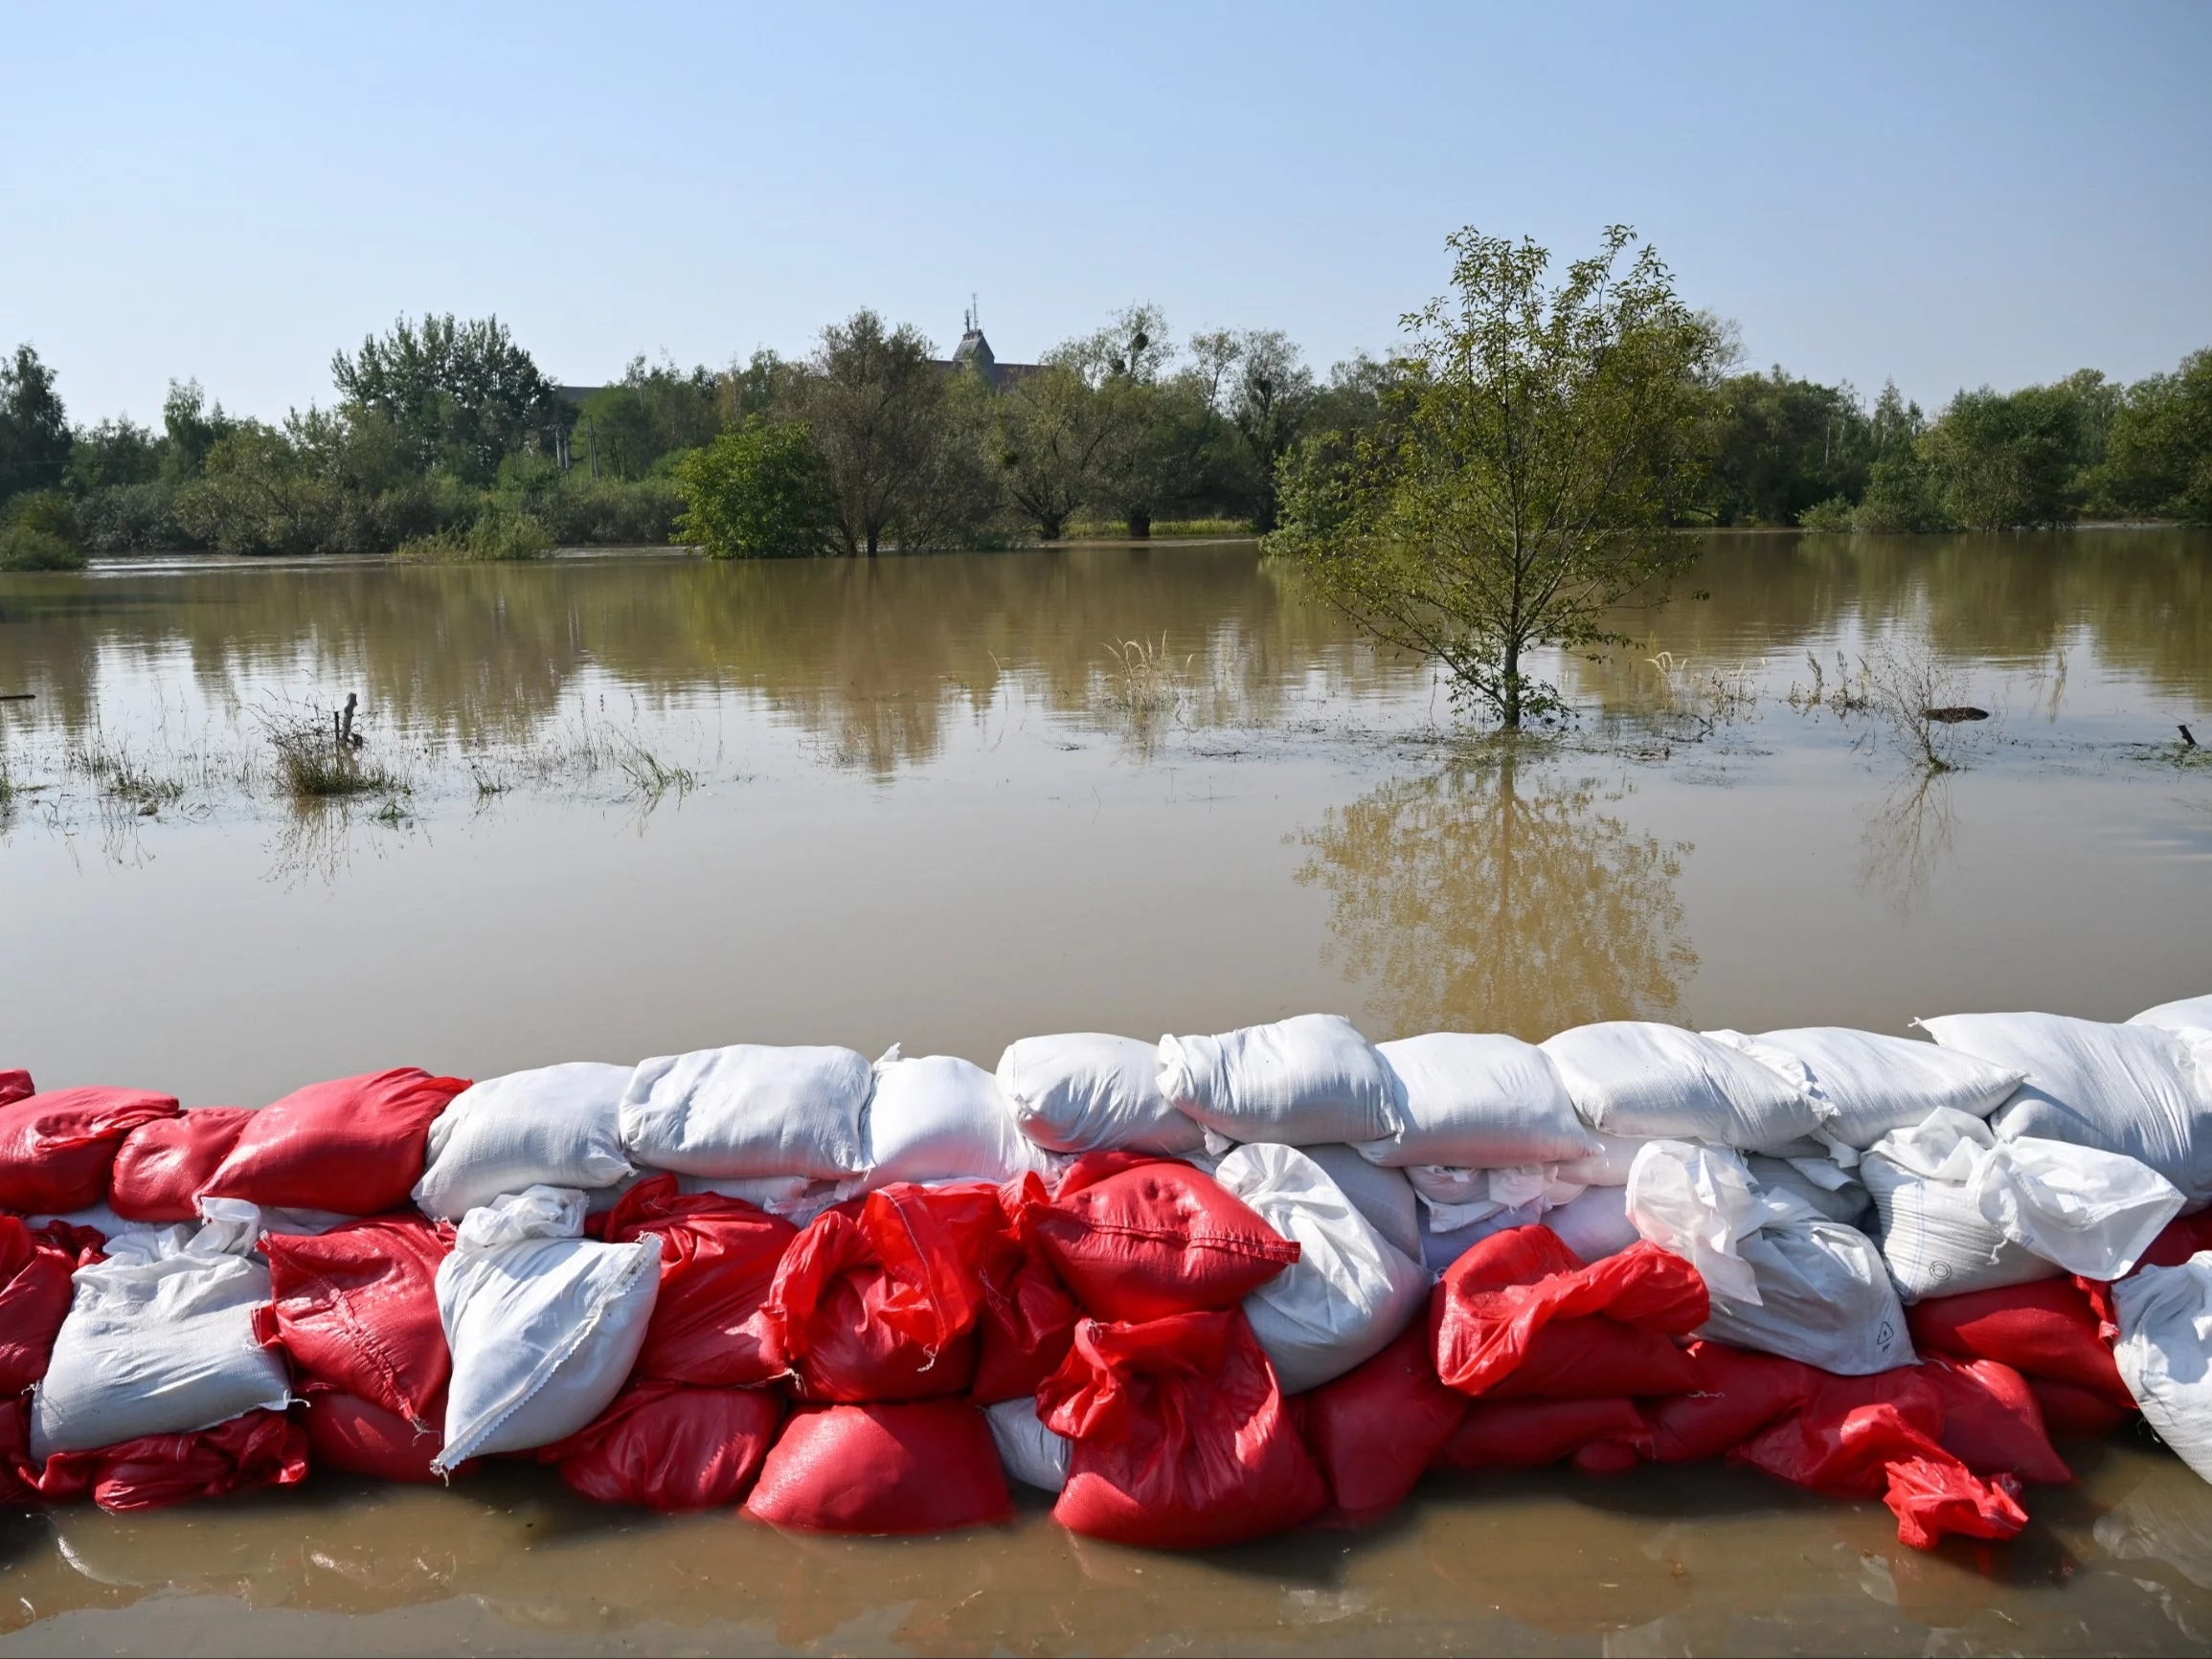
\includegraphics[width = 0.3\textwidth]{Pics/Dataset/przyklad_pelne_zdjecie.jpg}\label{fig:dataset_full_image}}
    \quad
    \subfloat[][Kafelek $640 \times 640$]{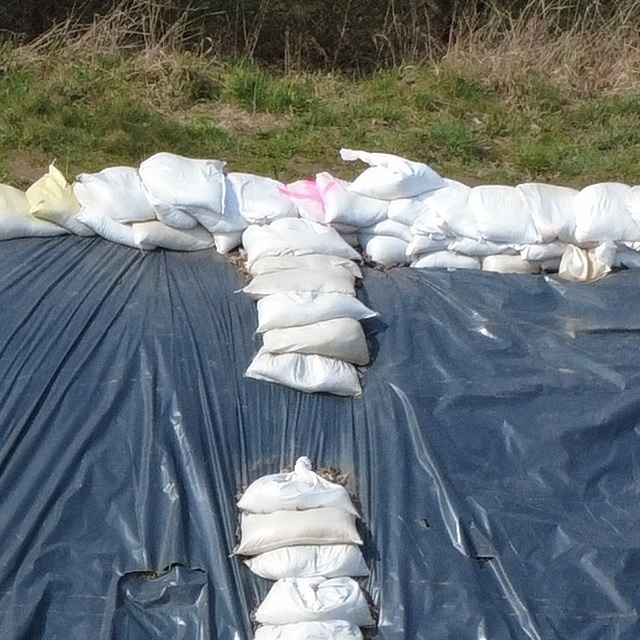
\includegraphics[width = 0.3\textwidth]{Pics/Dataset/przyklad_kafelek.jpg}\label{fig:dataset_tile}}
    \quad
    \subfloat[][Kafelek z~adnotacjami]{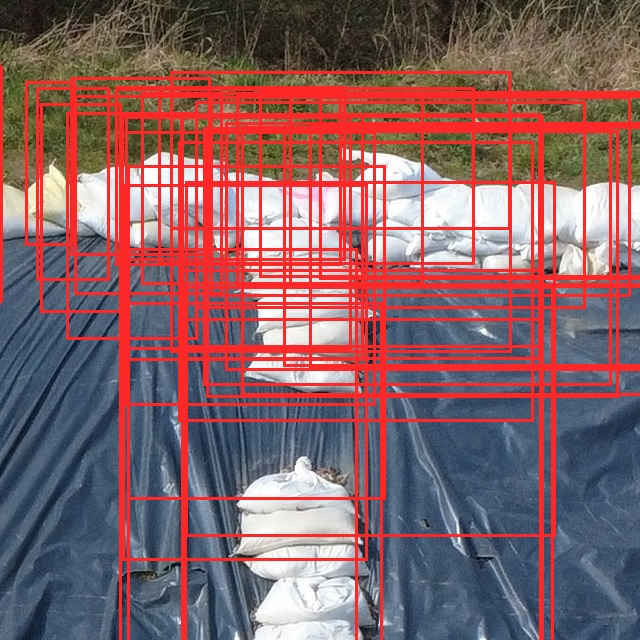
\includegraphics[width = 0.3\textwidth]{Pics/Dataset/przyklad_kafelek_adnotacje.jpg}\label{fig:dataset_tile_annotations}}
    \caption{Przykład przygotowania danych: od pełnego zdjęcia źródłowego do kafelka treningowego oraz odpowiadających mu adnotacji w~formacie detekcyjnym.}
    \label{fig:dataset_preparation_example}
\end{figure}

\subsection{Podział zbioru danych i~metodyka walidacji}

Na potrzeby prowadzonych badań, wygenerowane kafelki obrazu zostały rygorystycznie podzielone na trzy niezależne podzbiory o~ściśle określonych funkcjach:
\begin{enumerate}
    \item \textbf{Zbiór Treningowy (ang.\ \emph{Train}):} Zbiór liczący 171 oznaczonych próbek, wykorzystywany bezpośrednio do obliczania gradientów i~aktualizacji wag w~trakcie uczenia sieci.
    \item \textbf{Zbiór Walidacyjny (ang.\ \emph{Val}):} Niezależny zbiór oznaczonych obrazów, liczący 43 próbki, niebiorący udziału w~aktualizacji wag. Służył on do bieżącego wyliczania funkcji straty (ang.\ \emph{validation loss}) oraz wartości metryk (w~tym mAP) po każdej epoce. Na jego podstawie architektura decydowała o~zapisaniu optymalnego punktu kontrolnego (tzw.\ wagi \emph{best.pt}) przed nadejściem przeuczenia. To z~tego zbioru pochodzą wartości liczbowe analizowane w~wynikach ilościowych pracy.
    \item \textbf{Zbiór Testowy-Sacred (ang.\ \emph{Test-Sacred}):} Całkowicie wyizolowany zbiór referencyjny składający się z~23 próbek, do którego model nie miał dostępu na żadnym z~etapów treningu ani walidacji. Zbiór ten stanowi test zdolności do generalizacji na nowych domenach obrazowych i~został zarezerwowany wyłącznie do końcowej oceny jakościowej i~wizualnej.
\end{enumerate}

\subsection{Proces generowania pseudoetykiet (Metoda A)}

Zautomatyzowany proces uczenia oparty na generowaniu pseudoetykiet zrealizowano w~trybie iteracyjnym, zgodnie z~następującą procedurą:
\begin{enumerate}
    \item \textbf{Generowanie etykiet z~filtracją jakościową:} Model odniesienia (Nauczyciel) dokonywał predykcji na zbiorze nieoznakowanym. W~celu ograniczenia zjawiska błędu potwierdzenia (ang.\ \emph{confirmation bias}), akceptowano wyłącznie predykcje, dla których pewność modelu przekraczała empirycznie wyznaczony próg ($Conf \geq 0.45$). Odrzucano również detekcje o~anomalnie dużej powierzchni (powyżej $35\%$ kafelka), co stanowiło filtrację geometryczną eliminującą fałszywe wskazania w~obszarach tła.
    \item \textbf{Generowanie próbek negatywnych (ang.\ Negative Samples):} Obrazy niespełniające powyższych kryteriów oznaczano jako puste tło, co wymuszało na detektorze naukę poprawnego ignorowania obszarów takich jak niebo czy woda.
    \item \textbf{Uczenie Studenta z~zaszumieniem (ang.\ Noisy Student):} Model ucznia (inicjowany oryginalnymi wagami) trenowano na połączonym zbiorze danych z~wymuszeniem silnej augmentacji określonej w~pliku konfiguracyjnym. Wymuszało to uczenie bardziej ogólnych cech obiektów.
    \item \textbf{Kaskada iteracyjna:} Wynikowy wariant ucznia stawał się ulepszonym nauczycielem w~kolejnej pętli, podnosząc sukcesywnie jakość generowanych pseudoetykiet.
\end{enumerate}

\subsection{Syntetyzowanie próbek negatywnych (Metoda B)}

Alternatywnym podejściem uodporniania modeli na błędy detekcji była syntetyczna augmentacja obrazu. Do generowania czystych próbek tła (ang.\ \emph{negatives}) wykorzystano architekturę probabilistyczną \textbf{Stable Diffusion v1.5}. Proces wnioskowania zrealizowano lokalnie, wykorzystując bibliotekę \texttt{diffusers} oraz akcelerację GPU przy połowicznej precyzji zmiennoprzecinkowej (FP16).

Wykorzystując odpowiednio przygotowane zapytania tekstowe (ang.\ \emph{prompt engineering}), zaprojektowano warianty środowisk odpowiadające rzeczywistym danym z~drona (m.in.\ polany, drogi leśne z~lotu ptaka, place budowy). Generowane obrazy z~założenia nie zawierały obiektów docelowych, dzięki czemu system automatycznie przypisywał im pustą etykietę. W~standardzie YOLO i~RT-DETR taki plik stanowi jawną informację o~braku obiektu, na skutek czego funkcja straty silnie karze sieć za próby fałszywych detekcji. Na rysunku \ref{fig:gen_negatives} zaprezentowano przykłady otrzymanych próbek syntetycznych.

\begin{figure}[ht]
    \centering
    % Pierwszy rząd
    \subfloat[][Wyschnięta ziemia]{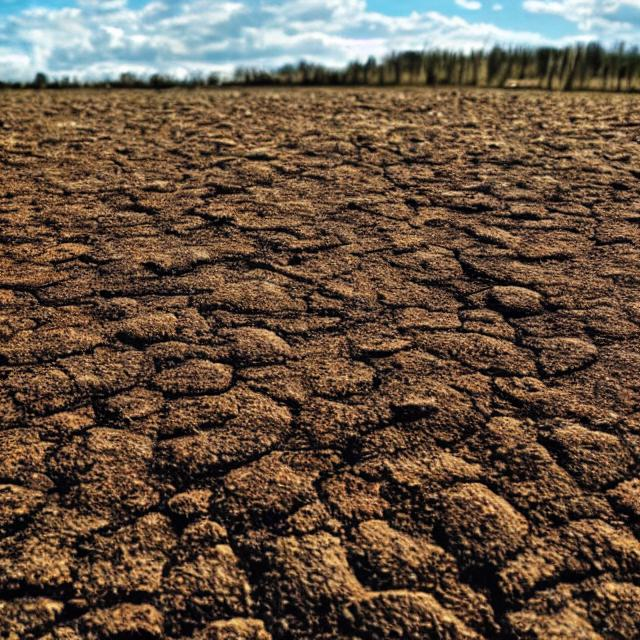
\includegraphics[width = 0.45\textwidth]{Pics/Generative_negatives/gen_neg_P1_001.jpg}\label{fig:gen_neg1}}
    \quad
    \subfloat[][Leśna droga z~drona]{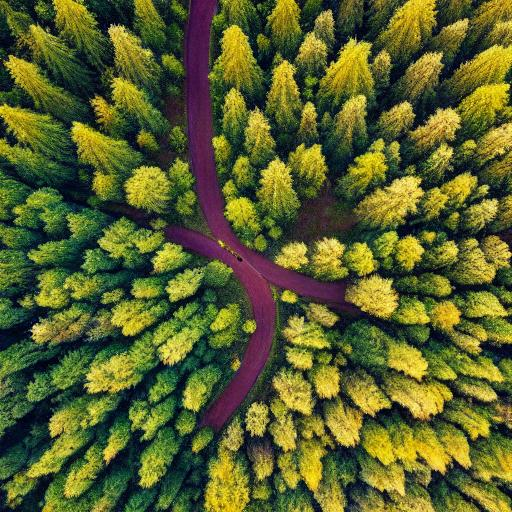
\includegraphics[width = 0.45\textwidth]{Pics/Generative_negatives/gen_neg_P2_009.jpg}\label{fig:gen_neg2}}
    
    \vspace{0.3cm} % Delikatny odstęp między rzędami
    
    % Drugi rząd
    \subfloat[][Plac budowy]{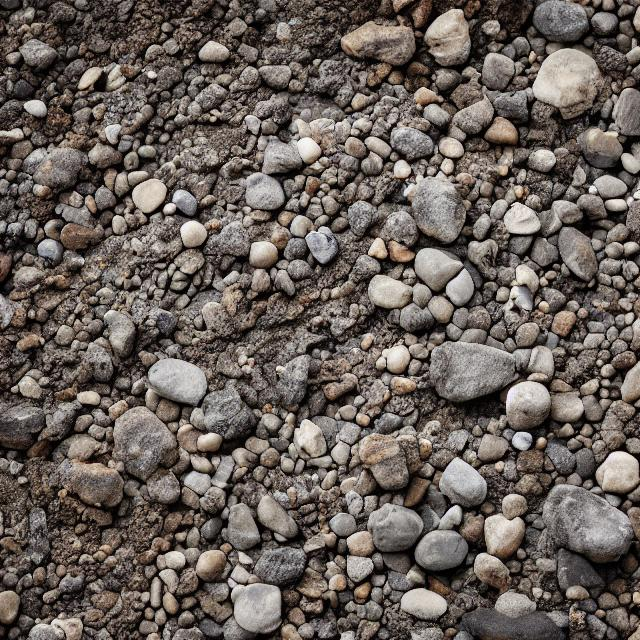
\includegraphics[width = 0.45\textwidth]{Pics/Generative_negatives/gen_neg_P3_033.jpg}\label{fig:gen_neg3}}
    \quad
    \subfloat[][Wał przeciwpowodziowy]{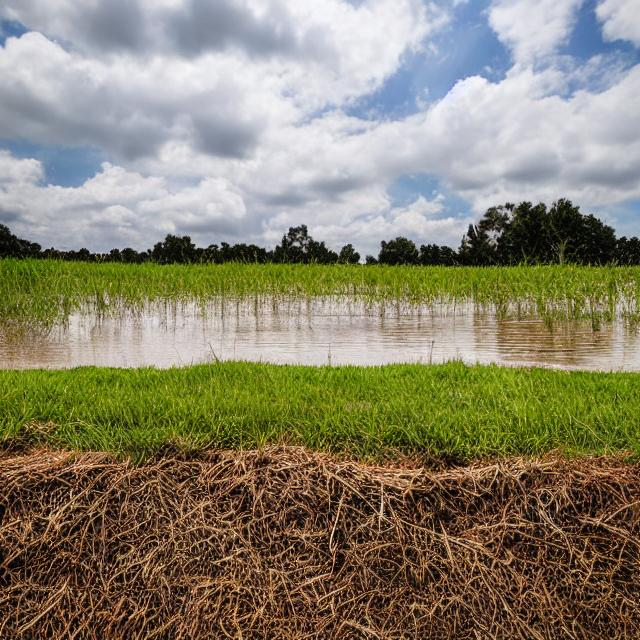
\includegraphics[width = 0.45\textwidth]{Pics/Generative_negatives/gen_neg_P5_062.jpg}\label{fig:gen_neg4}}
    
    \caption{Przykładowe syntetyczne próbki negatywne (tło bez obiektów docelowych) wygenerowane za pomocą modelu Stable Diffusion w~celu redukcji fałszywie pozytywnych detekcji.}
    \label{fig:gen_negatives}
\end{figure}

\section{Podsumowanie rozdziału}

W~rozdziale przedstawiono założenia metodologiczne oraz środowisko eksperymentalne wykorzystane w~badaniach. Zaprezentowano autorskie środowisko uruchomieniowe osadzone na klasterze obliczeniowym NVIDIA DGX, umożliwiające realizację procesu treningu dla modeli typu YOLO oraz RT-DETR. Zdefiniowano również sposób pracy z~ograniczonym zbiorem danych, ustanawiając podział na pule uczące, walidacyjne oraz wyizolowaną pulę \emph{Test-Sacred} do dodatkowej oceny wizualnej zdolności generalizacji.
